% vim:set et sw=2 ts=4 tw=72:
\chapter{Evaluation}

In June 2017, I conducted a study to quantitatively and qualitatively
evaluate the effectiveness of the visualizations and summaries presented
in \tool{} to the DAG-based visualizations found in Gitk and the git
command-line. The study was performed in a controlled environment
running Ubuntu 14.04. Participants were allowed to use Gitk and the git
command-line tools for these tasks, I will refer to both tools as Gitk,
when working with DAG-based visualizations and summarizations. I
considered allowing participants to use any of the free tools for Linux
suggested on the git
website\footnote{\url{https://git-scm.com/download/gui/linux}}, but
after attempting to use them, I found that none were able to operate on
repositories that were as large as the Linux repository. \tool{} was
used for evaluating the \mt{-based} visualizations.

The study has two primary goals; first determining if the DAG-based
visualization is sufficient for conceptual understanding, second
comparing \tool and Gitk to determine which is more capable of providing
users with a summarization of various metrics involved with integrating
a commit into the repository. These were done in two parts of the same
study. They were performed together as a single study for pragmatic
reasons, but could have been done as separate studies.

\section{Methodology}\label{sec:methodology}

This section describes the evaluation, how it was performed, the methods
used to ensure that things were kept consistent between participants,
and setting of the study. The evaluation was performed as a single
study, broken into two parts, using the same 12 participants and same 2
commits. The first part of the evaluation only used Gitk, while the
second part used Gitk and \tool{}. The order that the participants
studied each commit was randomized for each participant, but was kept
consistent through each part of the study. Participants would complete
part 1 of the study on both commits, the continue with part two, before
answering a few questions about their opinions and experience in an exit
survey. A screencapture with audio was taken for the duration of the
study with each participant. The videos were later analyzed and had the
information extracted into a more usable form.

Order bias was mitigated throughout the study through the use of
randomization between participants. In both parts, the order that the
participants worked with the commits, tasks, and tools was randomized.
More details about how this is done for each part are discussed in
Section~\ref{ssec:conceptual_study} and~\ref{ssec:summarization_study}.

Prior to starting the study, participants were given a quick
introduction to Gitk and Linvis, and could ask questions about either
interface. These introductions usually lasted no more than 10 minutes.
The goal was to test the visualizations and summarizations provided by
the tools, not the interface itself. Following the introduction to the
tools, I introduce the concept of the merge-tree, giving two examples,
shown in Figure~\ref{fig:DAG_to_MergeTree}, of how to convert between
the DAG and merge-tree, answering any questions that may arise.

\begin{figure}[htpb]
  \begin{center}
    \begin{tabular}{cc}
      \begin{tikzpicture}[auto, on grid, semithick,
        commit/.style={draw,shape=circle,fill=black}]
        \node[commit] (A) {};
        \node[commit, below right = of A] (1) {};
        \node[commit, below = of 1] (2) {};
        \node[commit, below = of 2] (3) {};
        \node[commit, below left = of 3] (I) {};

        \node[left = 0.5cm of A] {A};
        \node[right = 0.5cm of 1] {1};
        \node[right = 0.5cm of 2] {2};
        \node[right = 0.5cm of 3] {3};
        \node[left = 1.0cm of I] {Initial};

        \draw (A) edge[-stealth] (I) edge[-stealth] (1)
              (1) edge[-stealth] (2)
              (2) edge[-stealth] (3)
              (3) edge[-stealth] (I);
    \end{tikzpicture}
    &
    \begin{tikzpicture}[auto, on grid, semithick,
      root/.style={draw, circle, minimum size=0.8cm},
      leaf/.style={draw, circle, minimum size=0.8cm}]
      \node[root] {A}
      child {node[leaf] {1}}
      child {node[leaf] {2}}
      child {node[leaf] {3}};
    \end{tikzpicture}
    \\\midrule
    \begin{tikzpicture}[auto, on grid, semithick,
        commit/.style={draw,shape=circle,fill=black}]

        \node[commit] (A){};
        \node[commit, below right = of A] (1) {};
        \node[commit, below = of 1] (B) {};
        \node[commit, below = of B] (2) {};
        \node[commit, below = of 2] (3) {};
        \node[commit, below right = of B] (4) {};
        \node[commit, below left = of 3] (I) {};

        \node[left = 0.5cm of A] {A};
        \node[right = 0.5cm of 1] {1};
        \node[left = 0.45cm of B] {B};
        \node[left = 0.45cm of 2] {2};
        \node[left=0.45cm of 3]{3};
        \node[right=0.5cm of 4] {4};
        \node[left=1.0cm of I] {Initial};

        \draw (A) edge[-stealth] (I) edge[-stealth] (1)
              (1) edge[-stealth] (B)
              (B) edge[-stealth] (2) edge[-stealth] (4)
              (2) edge[-stealth] (3)
              (4) edge[-stealth] (3)
              (3) edge[-stealth] (I);
    \end{tikzpicture}
    &
    \begin{tikzpicture}[auto, on grid, semithick,
      every node/.style={draw, circle, minimum size=0.8cm}]
      \node {A}
      child {node {1}}
      child {node {B} child {node {4}}}
      child {node {2}}
      child {node {3}};
    \end{tikzpicture}
    \end{tabular}
  \end{center}
  \caption{Two examples of DAG to \mt{} conversions used in explanation
  during evaluation}
\label{fig:DAG_to_MergeTree}
\end{figure}

Two commits are used in both the conceptual study and summarization
study, with the goal of determining how well the DAG and \mt{}
visualizations scale between merges integrating varying numbers of
commits. The order that the two commits are presented to each
participant is randomized. I analyzed 15096 merge-trees from the
database that were candidates for the study, from April 16th 2005 to
October 14th 2014, corresponding to Linux releases 2.6.12-rc3 to
3.17-rc1. A merge-tree could only be selected if it was not a foxtrot,
and had correctly been identified. 25\% of the trees contain at most a
single repository event, not including the root, while 50\% of the trees
contain at most seven nodes. 75\% of the trees contain at least 51
nodes, and the largest tree contains 7217 nodes. 8031 trees contained at
least seven nodes, of these only 593 contained at least a single
internal merge node. Trivially, trees with a single node cannot have any
internal merge nodes. Of the 624 trees with seven non-root node, only
135 contained at least one inner node. Using this information, I chose a
random tree from the 2008 trees in the first quartile, which merges a
single commit into the master branch. These trees are trivial, but
appear frequently in the repository. The second tree was chosen randomly
from trees in the second quartile. These trees contain seven nodes, and
to increase the complexity of the tree, I required that the tree contain
at least one internal merge node.

Once the trees were selected, I had to select a commit from the tree.
Selecting a commit from the small tree was trivial, there was only a
single node to choose. From the medium-sized tree, I used a script to
select a commit randomly. The commits selected from the small tree and
medium tree were \emph{a3c1239eb59c0a907f8be5587d42e950f44543f8} and
\emph{cdbdd1676a5379f1d5cbd4d476f5e349f445befe} respectively. Commit 1,
the commit from the small tree is visualized in
Figure~\ref{fig:commit_1_visualization}, showing the DAG visualization
by Gitk and \rt{} tree visualization in Linvis. The same is
shown for commit 2 in Figure~\ref{fig:commit_2_visualization}.

\begin{figure}[htpb]
  \centering
  \begin{tabular}{cc}
    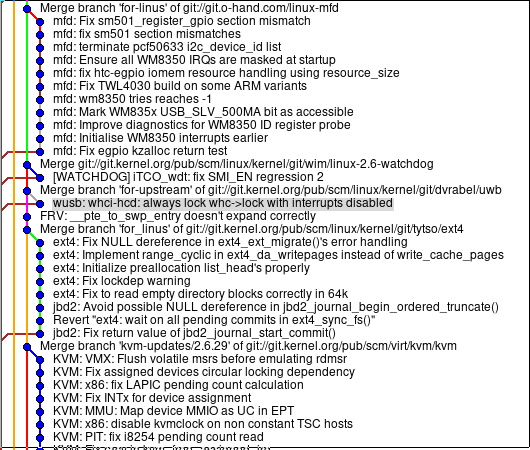
\includegraphics[height=4.5cm]{Figures/evaluation/commit1_gitk.png} &
    
\includegraphics[height=4.5cm]{Figures/evaluation/commit1_linvis.pdf}
  \end{tabular}
  \caption{The visualizations of commit 1 by Gitk and Linvis
    respectively.}
  \label{fig:commit_1_visualization}
\end{figure}

\begin{figure}[htpb]
  \centering
  \begin{tabular}{cc}
    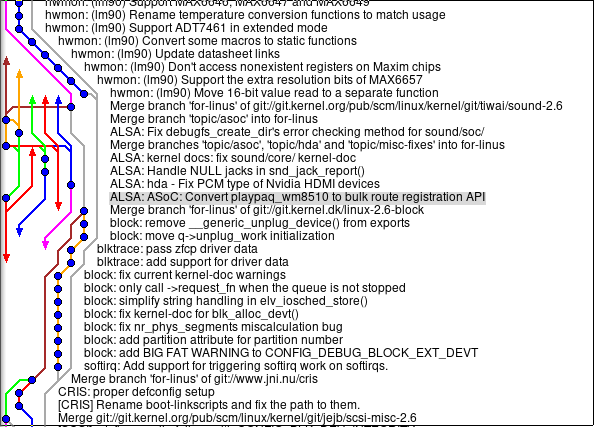
\includegraphics[height=4.5cm]{Figures/evaluation/commit2_gitk.png} &
    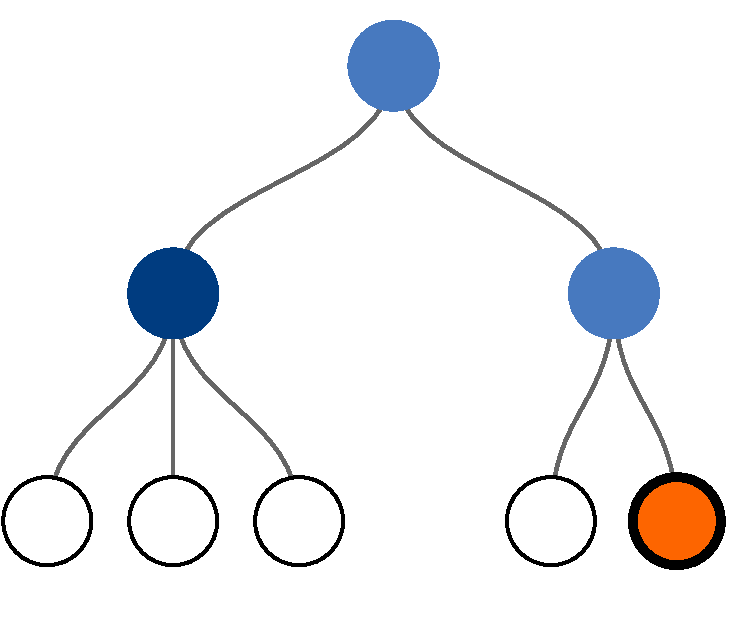
\includegraphics[height=4.5cm]{Figures/evaluation/commit2_linvis.pdf}
  \end{tabular}
  \caption{The visualizations of commit 2 by Gitk and Linvis
    respectively.}
  \label{fig:commit_2_visualization}
\end{figure}
